% 图 6.19 180 度畴壁与 90 度畴壁示意
\documentclass[tikz,border=5pt]{standalone}
\usetikzlibrary{arrows.meta}
\usepackage{amsmath}
\usepackage{bm}
\usepackage{fontspec}
\setmainfont{Times New Roman}
\begin{document}
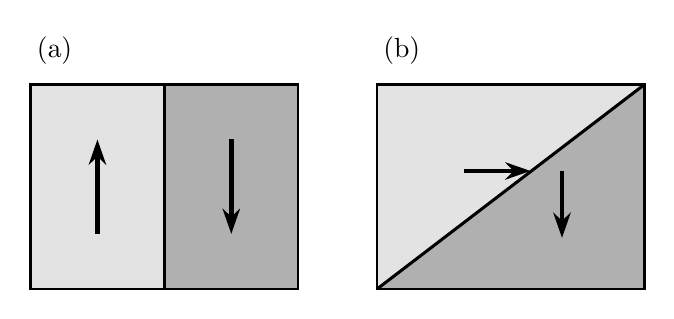
\begin{tikzpicture}[line width=0.8pt,>=Stealth,
  mag/.style={->,line width=1.6pt,>={Stealth[length=3.2mm,width=2.2mm]}}]
% ---------- (a) 180 degree wall ----------
\fill[gray!22] (0,0) rectangle (1.7,2.6);
\fill[gray!62] (1.7,0) rectangle (3.4,2.6);
\draw[line width=0.9pt] (0,0) rectangle (3.4,2.6);
\draw[line width=1.1pt] (1.7,0) -- (1.7,2.6);
\draw[mag] (0.85,0.7) -- (0.85,1.9);
\draw[mag] (2.55,1.9) -- (2.55,0.7);
\node[anchor=south west] at (-0.05,2.72) {(a)};
% ---------- (b) 90 degree wall ----------
\begin{scope}[shift={(4.4,0)}]
  \fill[gray!22] (0,0) -- (0,2.6) -- (3.4,2.6) -- cycle;
  \fill[gray!62] (0,0) -- (3.4,0) -- (3.4,2.6) -- cycle;
  \draw[line width=0.9pt] (0,0) rectangle (3.4,2.6);
  \draw[line width=1.1pt] (0,0) -- (3.4,2.6);
  \draw[mag] (1.1,1.5) -- (1.95,1.5);
  \draw[mag] (2.35,1.5) -- (2.35,0.65);
  \node[anchor=south west] at (-0.05,2.72) {(b)};
\end{scope}
\end{tikzpicture}
\end{document}
